Para comenzar a detallar el desarrollo realizado considero necesario hacer una introducción a algunos conceptos que tendrán importancia durante el transcurso del presente documento en relación con la física del sonido y la teoría musical, para facilitar la comprensión del documento a un lector no especializado en estos ámbitos. El capítulo tercero de \cite{Instinto} contiene gran información al respecto que solo se encuentra aquí a modo de resumen. 

\section{Fundamentos del sonido y teoría musical}
En primer lugar cabe destacar que como cualquier fenómeno físico, un sonido lleva asociados una serie de parámetros matemáticos que lo definen. Sin embargo, estos términos han recibido otro nombre en el ámbito musical debido a la tradición, con el que se enseñan en escuelas y conservatorios. Es importante, por tanto, tener clara la relación entre la nomenclatura musical y la equivalencia física y matemática.
\begin{itemize}
\item \textbf{Tono:} hace referencia a la altura de la nota en cuanto a grave o aguda por lo que el parámetro que la define es la frecuencias. Aunque el oído humano puede llegar a percibir señales de hasta 20kHz, las notas fundamentales producidas por instrumentos comunes rara vez sobrepasan los 2kHz.
\item \textbf{Volumen:} equivale a la intensidad que posee la señal tanto eléctricamente como cuando se propaga por el aire como una onda de presión. Cuando se mide en un circuito eléctrico se utilizan unidades de tensión mientras que como onda acústica se utilizan los dB dado su carácter logarítmico, no obstante, posee unidades de intensidad acústica: $W/m^{2}$.
\item\textbf{Timbre:} es característico de cada fuente de sonido y es lo que nos permite diferenciar un instrumento de otro -o voces humanas entre si- aún produciendo la misma nota.
\end{itemize}

La lista superior muestra los tres parámetros fundamentales de un sonido musical, sin embargo, no queda claro como funciona el mecanismo matemático que rige el funcionamiento del más relevante de ellos en este caso: el timbre.

\subsection{Timbre, armónicos y serie armónica}
Un estudiante de ingeniería está familiarizado con la generación de armónicos en el contexto de la física y las vibraciones. Sin embargo, puede que uno no se haya preguntado como se \emph{oyen} estos modos o si se pueden percibir. La respuesta es sí, y además con mucha claridad \cite{arm_wood}. En lo que se refiere a la música, tanto los instrumentos musicales como la voz humana son estructuras complejas que producen sonidos a muchas frecuencias diferentes al mismo tiempo. Nuestro cerebro, cuando oye un sonido, se encarga de interpretar la señal recibida para relacionarla con un sonido identificable. 

Es inevitable y necesario establecer una analogía entre este funcionamiento y el teorema de Fourier, que a grandes rasgo expresa que siempre se puede descomponer cualquier señal como suma de una o varias componentes sinusoidales. Esta poderosa afirmación explica como funciona la generación de cualquier sonido musical .

Así pues, cuando se produce una nota con un instrumento, se generan varias vibraciones a distintas frecuencias, en consecuencia, es la relación entre estas componentes la que modifica el timbre de la nota generada y nos permite identificar el sonido adecuadamente \cite{arm_str}. La trampa está en que las frecuencias que se producen no son generalmente aleatorias, si no que son un conjunto de notas concretas que reciben el nombre de \emph{armónicos}. La agrupación de estos armónicos recibe el nombre de \emph{serie armónica}.

\begin{figure}[!b]
\begin{center}
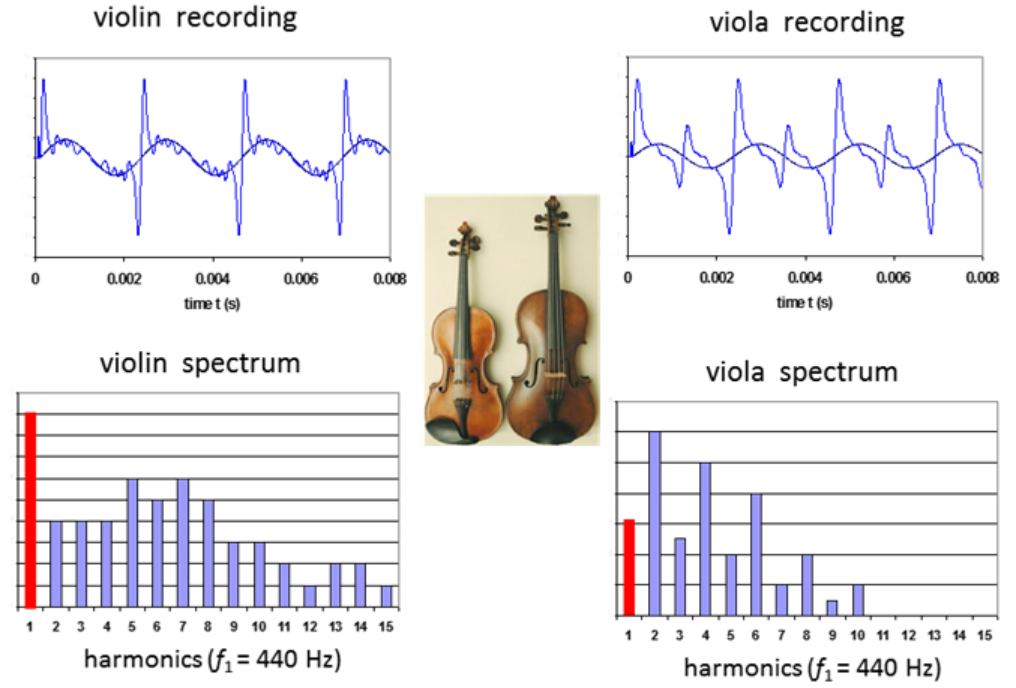
\includegraphics[width=14cm]{img/armonicos.png}
\caption{\label{fig:armonicos}Comparativa de una nota en dos instrumentos. En rojo la fundamental.}
\end{center}
\end{figure}

Así pues, podemos concluir que cada nota está a su vez formada por varios armónicos, presentándose en diferente proporción entre ellos. El armónico que define el sonido es el primero de la serie, llamado fundamental. El resto se obtienen (idealmente \cite{arm_wood2}) multiplicando la frecuencia de este por los distintos números enteros. En la imagen \ref{fig:armonicos} se muestra una comparativa de las diferencias, a nivel de serie armónica, que existen entre un violín y una viola cuando interpretan ambos la misma nota. Las operaciones que vamos realizar en la señal de entrada tienen como objetivo modificar el tono de una nota introducida mientras mantenemos inalterados su volumen y su timbre. En la práctica se comprobará como tanto el algoritmo como el procesado en la FPGA introducen desviaciones y no idealidades que nos permiten elaborar y clasificar diferentes métodos y operativas.

\section{Aproximaciones a la octavación}
En general, el propósito de un octavador es proporcionar una señal una octava inferior a la señal introducida. En consecuencia el algoritmo debe dividir la frecuencia de cada muestra entrante por dos. Lo primero que salta a la vista es la manifiesta relación con la transformada de Fourier para operar en el dominio de la frecuencia, sin embargo, el coste computacional y temporal de implementar esta operación matemática es elevado. Es por ello que se estudian diferentes posibilidades que pudiesen simplificar la arquitectura.

El primer pensamiento es que se trata de algo sencillo: basta con eliminar una de cada dos muestras en el espectro, es decir, un diezmado en frecuencia por un factor 2, para obtener a la salida una señal con las frecuencias divididas tal como se persigue \cite{Oppenheim}. A pesar de que las propiedades de la transformación hacen imposible realizar esta operación, debido a que las frecuencias de entrada son numerosas y variables no basta este diezmado, ya que el desajuste en la fase produce un desplazamiento circular en la señal de salida (ecuación~\ref{eq:DESP}). 

\begin{equation}
\label{eq:DESP}
Si~~~~~\mathscr{F}(\{x_{n}\})_{k} = X_{k}~~~~~Entonces~~~~~\mathscr{F}(\{x_{n}e^{\frac{2\pi i}{N}nm}\})_{k}= X_{k-m} 
\end{equation}

La consecuencia es que si la señal de entrada no es una única nota invariante, la salida resulta irreconocible, por lo que hay que descartar inmediatamente este proceder. Otra consideración que no hay que dejar de lado es la pretensión de operar en tiempo real. Esto supone que se debe tener en cuenta un mecanismo que permita \emph{trocear} la señal en conjuntos finitos para poder aplicar la transformación de Fourier. Este proceso, junto con la propia implementación de la transformada va a complicar en gran medida la arquitectura, es por ello que se decide en primer lugar evaluar los algoritmos que no precisan de esta operativa.

\subsection{Prescindiendo de Fourier}
\label{nofourier}
De cara a obtener un pedal de efectos para un instrumento más grave, se podría haber pensado en optar por un octavador ascendente. Esto, aunque parece que plantea los mismos problemas, resulta mucho más sencillo de implementar precisamente por ser 2 el factor de multiplicación. La fácil solución consiste en elevar cada muestra al cuadrado y realizar un filtrado pertinente que aísle las componentes en la zona del espectro adecuada, de forma que $x_{out} = x_{in}^{2}$. Consecuentemente, se produce un aumento llamativo de los armónicos produciendo una variación en el timbre que podría resultar o no conveniente, especialmente es intrumentos como el saxofón que ya generan un elevado número de armónicos. Este tipo de efectos recibe el nombre de \emph{enhancer} y pueden llegar a modificar el timbre de forma significativa. La operativa descrita anteriormente me fue sugerida por José Parera, al que agradezco el tiempo que me ha dedicado. Si añadiésemos a este otros efectos como tremolo, reverb o delay, podríamos realizar una aproximación muy válida a un pedal comercial, con todo, he preferido mantenerme fiel a la intención original de realizar la octavación descendente.

Pese a ello, merece la pena probar que ocurre si se realiza la operación opuesta, $x_{out} = \sqrt{x_{in}}$, de forma que se octave la señal de forma descendente. El resultado es menos halagüeño de lo que pudiera parecer, en primer lugar está el inconveniente de tener que lidiar con las muestras de valor negativo\footnote{Como se verá más adelante, el método de entrada en la FPGA devuelve las muestras normalizadas en el rango (-1,1)}, lo que resulta una molestia de cara al flujo de datos. Además, debido a que la entrada está limitada en banda, al reducir de forma cuadrática el valor de los armónicos más agudos, se produce una modificación en el timbre que provoca un sonido \emph{robótico} o \emph{artificial}. Por estas razones, se descarta este proceder.

La última de estas operativas \emph{sencillas} consiste en utilizar las propiedades de la multiplicación por coseno para modular la señal a la altura deseada. Aunque la idea parece simple, resulta muy complicada de llevar a la práctica porque habría que implementar un algoritmo que detectara los picos de frecuencia y los modulara utilizando un coseno de valor $f_{pico}/2$. La detección de picos de frecuencia ya supone la vuelta al dominio de Fourier, sin contar con que la gestión de la anchura de esos picos se hace muy compleja. No obstante, el algoritmo de baja latencia que se describe posteriormente en la sección~\ref{rhilbert} propone algo similar.

\subsubsection{Algoritmo NFC-TSM}
Siguiendo el consejo de José Parera, recurrí a \emph{dafx.com}, que se trata de una página dónde se publican anualmente un gran número de estudios relacionados con los efectos digitales de audio y de donde he obtenido la mitad de las referencias bibliográficas. De la investigación en esta página descubrí un algoritmo que realizaba la octavación descendente sin llevar a cabo la transformada de Fourier, descrito en \cite{nfctsm}.

Este documento propone un ingenioso algoritmo al que los autores llaman Modificación de Escala Temporal por Correlación Normalizada y Filtrada o por sus siglas en inglés \emph{NFC-TSM}. El esquema de funcionamiento es el siguiente; primeramente se lleva a cabo un remuestreo con la tasa deseada $f_{s_original}/f_{s_replay}$ (para realizar la octavación debería ser 2:1). En segundo lugar tiene lugar el proceso de la modificación de la escala temporal que vuelve a variar la escala para obtener una salida de igual tamaño que la entrada.

\begin{figure}[!ht]
\begin{center}
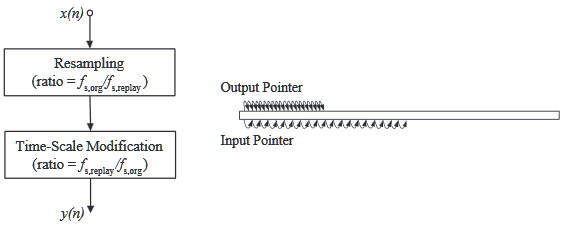
\includegraphics[width=12cm]{img/nfc-tsm.png}
\caption{\label{fig:tsm}Esquema del funcionamiento NFC-TSM en octavación descendiente}
\end{center}
\end{figure}

\begin{equation}
\label{eq:amdf}
D(m) =  \sum_{k = 0}^{L - 1}|~x(k+m)-x(k)~|
\end{equation}

En las propias palabras de los autores, la idea consiste en descartar y repetir algunos segmentos de la señal para comprimir o expandir la longitud del audio resultante. Utilizan para ello un sistema de buffer circular con dos punteros que se mueven a diferente velocidad añadiendo algunas variaciones para evitar una colisión entre ambos. En consecuencia, los saltos que lleva a cabo el puntero más rápido tienen longitud variable y pueden ser en cualquier dirección, puesto que la distancia entre los puntero no es fija. Además se calcula el mejor punto para realizar el salto mediate la función AMDF (ecuación \ref{eq:amdf}) para evitar una discontinuidad demasiado abrupta que resulte percetible al oído. 

A grandes rasgos, la función AMDF se utiliza para ajustar el salto del puntero de manera que no se rompa la periodicidad de la señal, la cual podría no mantenerse si el punto de salto fuera aleatorio. Para ello, se compara una ventana de correlación correspondiente a donde se ubica el puntero con un área de búsqueda determinada. El punto de salto se ubica siempre en el mínimo de la función AMDF para cada área de búsqueda. La longitud de las ventanas así como su ubicación son parámetros configurables del algoritmo, tal y como aclaran los autores.

En resumen, este método combina varias operativas para lograr un algoritmo versátil que puede variar al factor de octavación de forma flexible con una calidad relativamente buena en todos ellos. No obstante, para llevar a cabo la ejecución de esta manera es necesaria mucha capacidad de cálculo, ya que la AMDF requiere de numerosas operaciones\footnote{Estas se detallan en el artículo \cite{nfctsm} en varios escenarios diferentes}, haciéndolo poco deseable para un procesado en tiempo real, como es el caso. La siguiente solución presentada propone un concepto de cálculo más sencillo pero que se repite en muchas ocasiones, lo cual resulta mucho más deseable a la hora de introducirlo en la placa.

\subsubsection{Algortimo de baja latencia}
\label{rhilbert}

Para comprender la base de esta idea, descrita en profundidad en \cite{hilbert}, hay que diferenciar dos maneras de abordar la problemática del cambio de afinación a grandes rasgos, ya que existen dos maneras de hacerlo:
\begin{itemize}
\item \textbf{Desplazamiento de tono: }o \emph{pitch shifting}, se basa en que cada frecuencia se \textbf{multiplica} por una constante. Este el caso de los algoritmos descritos antes que pretendían dividir todas las frecuencias entre dos.
\item \textbf{Desplazamiento de frecuencia: }o \emph{frequency shifting}, en este caso se \textbf{suma} (o resta) a cada frecuencia una constante definida previamente. Estas técnicas no se han aplicado anteriormente en algoritmos de cambios de afinación porque se rompen las relaciones armónicas entre una fundamental y sus componentes. Sin embargo, la solución que proponen los autores para construir el algoritmo de baja latencia esta basada en este tipo de desplazamiento.

\end{itemize}
De forma equivalente a algunos métodos anteriores, si a cada frecuencia le restamos su frecuencia mitad, $f_{out} = f_{in}-f_{in}/2$, obtenemos un resultado idéntico a la división por dos. Este algoritmo se construye sobre esta idea, la cual, para que funcione, debe \emph{fijar} las frecuencias entrantes de alguna manera, ya que si no, no se puede conocer a priori qué constante hay que utilizar en cada momento. La solución es utilizar un banco de filtros IIR lo suficientemente estrechos como para que se distingan correctamente dos notas sucesivas. De esta forma, se realiza la resta inmediatamente después de haber hecho el filtrado, como se muestra en \ref{fig:fshil}. Conociendo la afinación del saxofón, se pueden conocer de antemano las frecuencias de entrada, por lo que habrá que centrar cada filtro con una de las notas del registro. El resto del espectro correspondiente a los armónicos se cubre con filtros equiespaciados siempre en escala logarítmica.

\begin{figure} [!h]
\begin{center}
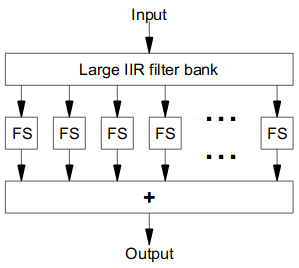
\includegraphics[width=7cm]{img/filtros_hilbert.png}
\caption{\label{fig:fshil}Algoritmo de baja latencia. FS equivale a cada etapa de desplazamiento en frecuencia}
\end{center}
\end{figure}

Tal y como proponen los autores es necesario que el ancho de banda de cada filtro vaya aumentando junto a la frecuencia, estableciendo un mínimo de 50Hz para las frecuencias más bajas. En esto radica uno de los problemas de este algoritmo: se produce inevitablemente una ligera desafinación que se puede acentuar si se pierde la relación entera con los armónicos superiores. Esta desafinación es más pronunciada en las frecuencias inferiores debido al ancho de banda mínimo establecidom, puesto que cada filtro se puede llegar a extender a varias notas.

Para realizar cada etapa de restado, son necesarios dos osciladores a 90º, una transformada de Hilbert y otros pocos componentes más, como ilustra la figura \ref{fig:restahil}. Adicionalmente, se puede sustituir la etapa de la transformada de Hilbert por filtros IIR, reduciendo aún más el coste computacional total. No obstante, es cierto que el elevado número de módulos, aunque sencillos, tienen un coste de área grande en la FPGA, aunque en ningún caso resulta crítico.

\begin{figure}[!t]
\begin{center}
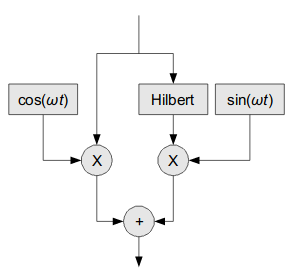
\includegraphics[width=7cm]{img/fs_hilbert.png}
\caption{\label{fig:restahil}Esquema de cada etapa de restado en el dominio del tiempo}
\end{center}
\end{figure}

La razón para no implementar este algoritmo de baja latencia ha sido puramente personal, ya que he priorizado eliminar el desafinamiento a reducir la latencia. En la fuente bibliográfica \cite{hilbert} hay muestras de audio de buena calidad comparando diferentes métodos, pero ninguno de ellos estaba implementado en FPGA. Aunque hubiera resultado interesante, probar este algoritmo en Matlab (no he encontrado ningún código ya realizado) hubiera requerido de mucho más tiempo para la parte de diseño que de implementación, cuando mi idea era centrarme más en esta última. Además, considero crítico el desafinamiento inherente a esta forma de cálculo que no se puede evitar de ninguna manera.

\subsection{Retorno a la transformada}
Así pues, se va a detallar la arquitectura basada en un \emph{Vocoder de fase} la cual será finalmente elegida para su implementación y se presenta en los epígrafes sucesivos. Esta es la aproximación más común a esta problemática y en ella se basan muchos de los productos comerciales disponibles en el mercado.

\section{Breve historia del vocoder}
Durante todo el siglo XX se han ido desarrollando diferentes técnicas de tratamiento y codificación para la voz, conforme iba la tecnología en aumento \cite{VocHis}. La consecuencia de ello es la aparición de diversos algoritmos que permiten este tipo de operaciones con una carga computacional relativamente baja. 

Un \emph{Vocoder}, del inglés \emph{voice} (voz) junto a \emph{encoder} (codificador), es generalemente cualquier aparato que analiza y/o sintetiza la voz humana para lograr  algún objetivo concreto, como compresión de datos, multiplexación o encriptación \cite{VocOvw}.

Concretamente, el Vocoder de canal\footnote{Del inglés \emph{channel vocoder}}, desarrollado por los famosos \emph{Bell Labs} en 1928, utilizaba varios filtros multibanda seguidos por detectores de envolvente cuyas señales de control se transmitían al decodificador del receptor. Estas señales de control son mucho más lentas que la señal original a transmitir, por lo que se puede reducir el ancho de banda permitiendo a un mismo medio de transmisión soportar un mayor número de canales, ya sea por radio o cable. Finalmente, el decodificador amplifica estas señales de control en destino, introduciéndolas en los filtros correspondientes a cada banda para poder sintetizar de nuevo la señal original. Además de las ventajas sobre el ancho de banda, también se ayuda a proteger la señal para que no se pueda interceptar. Encriptando las señales de control y modificando los parámetros de los filtros, se puede hacer muy difícil su correcta reinterpretación si no se sincronizan codificador y decodificador. Esto popularizó su uso durante la Segunda Guerra Mundial en el bando aliado, patentándose diversos diseños basados en estas ideas.

El concepto se ha mantenido constante durante todo el siglo hasta nuestros días, donde podemos ver implementaciones modernas de la misma idea, llegando incluso a desarrollarse una estandarización común a todos ellos. La voz humana posee un rango de frecuencias de entre 200 y 3400 Hz típicamente, optando por una frecuencia de muestreo de $8~kHz$ en consecuencia. Es común que se utilice una codificación con 16 bit por muestra por analogía con el estandar CD, pero con utilizar al menos 12 la mayoría de los receptores será capaz reproducir la señal con una fidelidad razonable. Citando un ejemplo, los codificadores según la norma ITU G.729, que son utilizados en telefonía comercial, tienen una buenísima calidad con una tasa binaria de 8 kbps. Actualmente, los vocoder también se utilizan para desarrollar tecnologías relacionadas con la lingüistica, la física y la neurociencia.

\subsection{Vocoder en la música}
Paralelamente a su utilización en comunicaciones, el vocoder se comenzó a popularizar durante la década de los 70 como método de síntesis, ya que esta estaba muy de moda en la época. Cabe mencionar, que durante esta década, surge un gran interés en los músicos por experimentar con diferentes timbres y sonidos en todo tipo de instrumentos: tradicionales o experimentales. Para aplicaciones musicales, se utiliza la frecuencia portadora proveniente de un instrumento en lugar de extraer la frecuencia fundamental del sonido que se esta grabando. El resultado es una deformación del sonido capturado que, por estar afinado en una nota adecuada, produce un resultado agradable al oído. Fue el primer fabricante de sintetizadores y pionero de la música electrónica, Robert Moog, el que desarrolló un prototipo llamado \emph{Farad} en 1968, pero no fue hasta 1970 cuando unieron el funcionamiento de esta máquina con el famoso sintetizador modular \emph{Moog} que se había lanzado previamente al mercado. Quedaba ya conformada la esencia de utilizar la señal proveniente de un micrófono como moduladora y la proveniente de sintetizador como portadora para modularla. Algunos ejemplos tempranos de músicos reconocidos que utilizaron estos dispositivos fueron Phil Collins, Mike Oldfield, Stevie Wonder, Herbie Hancock o Michael Jackson.

\begin{figure}
\begin{center}
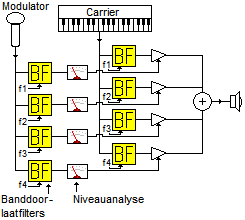
\includegraphics[width=8cm]{img/music_vocoder.png}
\caption{Esquema del funcionamiento de un vocoder musical}
\end{center}
\end{figure}

Estos vocoder proporcionaban sonidos a los que el público estaba poco acostumbrado porque realmente no mantenían una fidelidad tímbrica respecto el sonido que captaban. Por ello se empezaron a utilizar los vocoder de fase, los cuales permiten llevar a cabo expansión o compresión en el tiempo y  modificar la altura musical del sonido o afinación sin cambiar la forma de onda que proporciona el timbre característico.

El método para hacerlo es el siguiente. En primer lugar se lleva a cabo una transformada mediante STFT (Short Time Fourier Transform) para posteriormente modificar la afinación mediante sub y sobremuestro. Este proceso hace que el audio resultante no resulte reconocible, por lo que es necesario ajustar el valor de la fase de cada muestra para mantener la coherencia entre ellas, de ahí el nombre de vocoder de fase. Una vez calculadas las muestras, se transforman de vuelta al dominio del tiempo, donde se rellena con ceros para obtener una salida con la misma duración que la señal entrante. A continuación se explican en detalle estas etapas, basadas en el trabajo de D.Ellis descrito en \cite{Ellis}.

\section{Transformación a frecuencia: STFT}

Una STFT (Short Time Fourier Transform o Transformada de Fourier en Tiempo Corto) es en una manera especial de computar una transformada de Fourier y se usa para determinar el módulo y fase de muestras próximas de una señal mientras cambia con el tiempo, haciéndola muy adecuada para aplicaciones en tiempo real. Para ello, se divide la señal en segmentos más cortos de la misma longitud y se calcula la transformada de cada uno de ellos por separado. El método para calcular la transformada es indiferente pero para obtener una latencia lo suficientemente baja, conviene decantarse por el algoritmo de la Transformada Rápida de Fourier o FFT.

\subsection{Transformada de Fourier: FFT e iFFT}

Para realizar la transformación al dominio de la frecuencia, la opción más adecuada es sin duda el algoritmo de la FFT. Este algoritmo calcula la Transformada de Fourier en Tiempo Discreto o DFT descomponiendo la señal original de longitud $N$ en fragmentos de tamaño $N/2$ como muestra la figura~\ref{fig:fft} y  multiplicando posteriormente cada muestra por los términos constantes $W_{n}$ calculados previamente \cite{Oppenheim}. Nótese que en los bloques de $N/2$ se puede volver a aplicar el mismo principio de forma recursiva. Esto consigue reducir el tiempo de cálculo porque la transformada propiamente dicha se calcula para una longitud mucho menor, dados los coeficientes constantes. En la ecuación~\ref{eq:FFT} correspondiente la DFT genérica podemos ver como la complejidad depende cuadráticamente de la longitud de la entrada $O({n^{2}})$ mientras que la FFT lo computa únicamente con complejidad $O({n\cdot\log (n)})$.

\begin{figure}[!ht]
\begin{center}
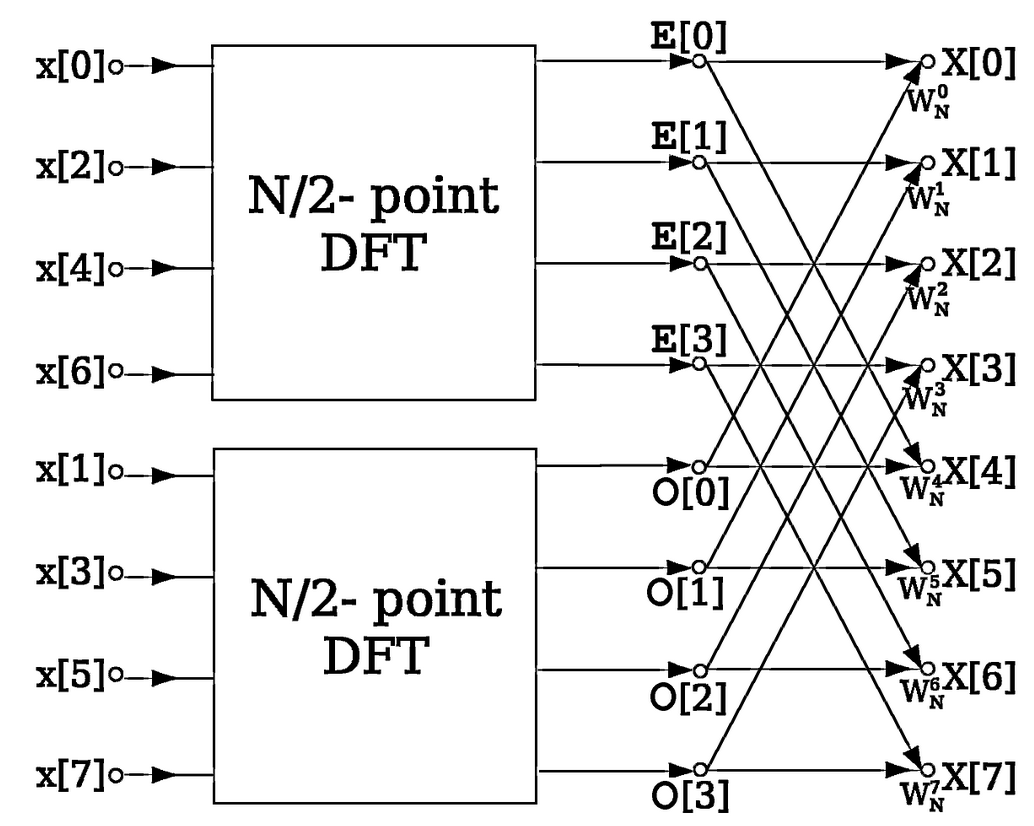
\includegraphics[width=10cm]{img/dft.png}
\caption{\label{fig:fft}Esquema del algoritmo para la realización de la FFT}
\end{center}
\end{figure}

\begin{equation}
\label{eq:FFT}
X(k) =  \sum_{n = 0}^{N - 1} x_{n}e^{-2\pi kni/N}~~~~~~~~Donde~~~~k = 0, 1...., N-1
\end{equation}
\begin{equation}
\label{eq:iFFT}
x(n) = \frac{1}{N} \sum_{n = 0}^{N - 1} X_{k}e^{-2\pi kni/N}~~~~~Donde~~~~n = 0, 1...., N-1
\end{equation}

El caso de la transformada inversa es totalmente análogo, el algoritmo de la FFT se puede aplicar de la misma forma para realizar iDFT de forma más rápida, lo que se conoce como iFFT. La ecuacion~\ref{eq:iFFT} muestra la expresión genérica de la iDFT para un señal de N muestras. Cada uno de los parámetros que se utilizan para realizar las transformaciones se encuentra explicado posteriormente en la sección \ref{ap:FFT}.

\subsection{Solapamiento y enventanado}

Dividir la señal entrante en sucesivas tramas es un proceso sencillo, únicamente se almacenan las muestras en una memoria para introducirlas posteriormente en el módulo que realiza la FFT. El problema entonces reside en la propia naturaleza de la misma, ya que esta funciona perfectamente para señales periódicas, pero al trocear la señal en pequeñas tramas, no se garantiza que estas tramas contengan un número entero de periodos. Esto se agudiza especialmente cuando la señal es variante con el tiempo y el número de elementos por trama es independiente de la frecuencia de la señal de entrada.

\begin{figure}[!ht]
\begin{center}
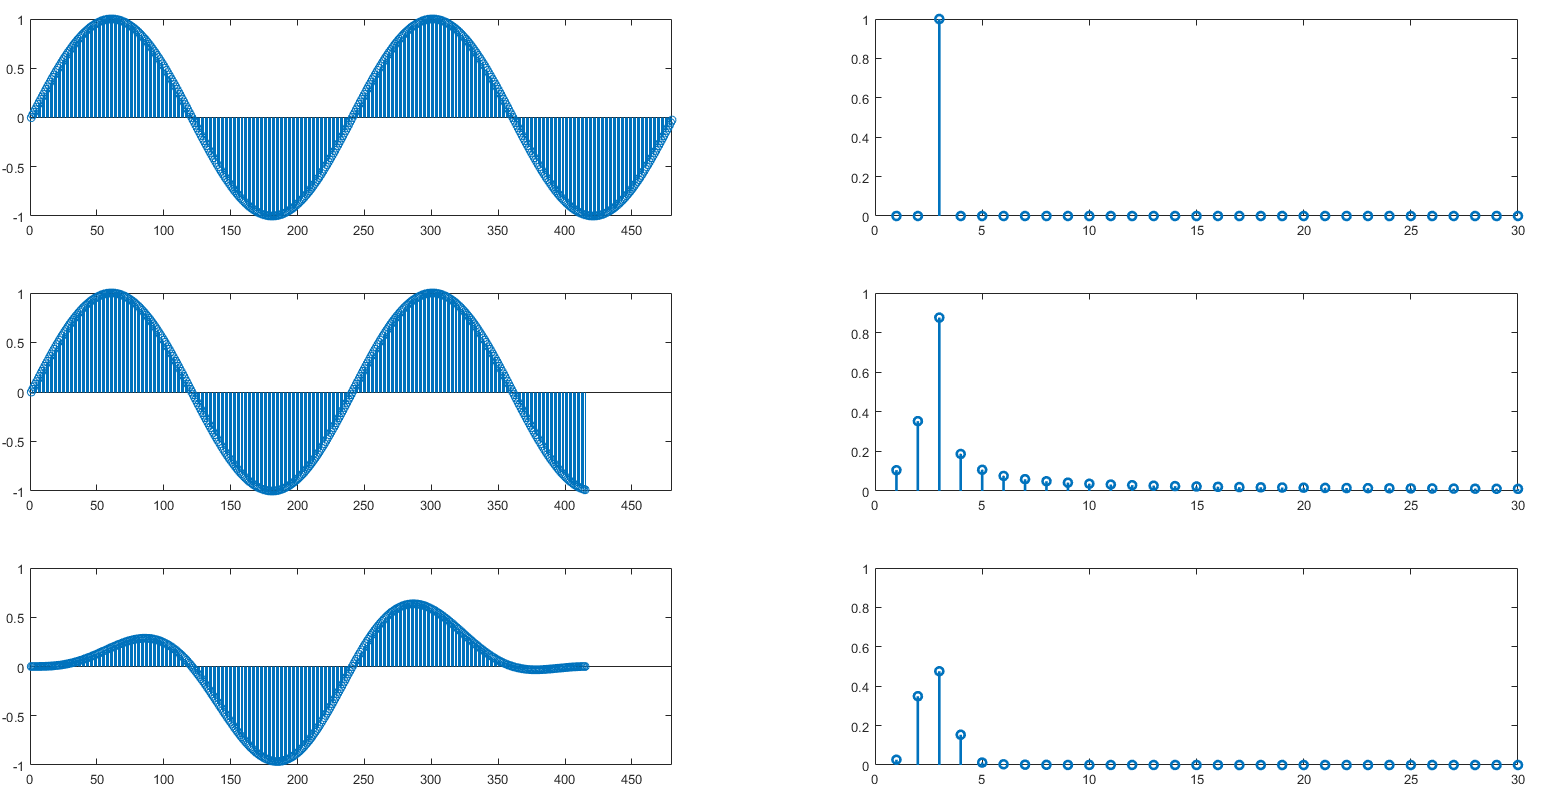
\includegraphics[width=14cm]{img/problem_fft.png}
\caption{\label{fig:probfft}Señal sinoidal y su FFT con periodos enteros, recortada y enventanada}
\end{center}
\end{figure}

En la figura~\ref{fig:probfft} se ilustra el problema del recortado arbitrario descrito y su mejora al aplicarle enventanado: al suavizar el salto de frecuencias, este resulta menos molesto al oído. Frente al caso ideal, el primero, el corte del segundo caso introduce componentes en otras frecuencias que se traducirán como un ruido molesto al final de cada trama, conocido en en inglés como \emph{clipping}. Podemos comprobar como al aplicar un enventanado a la señal de entrada, este se hace menor y afecta a menos muestras. Para este ejemplo se ha utilizado una ventana de Hann como la que se utilizará en el prototipo.

Junto al enventanado, se suele aplicar cierto \emph{solapamiento}, es decir, en lugar de empezar a construir una trama a continuación de la anterior, se comienza a llenar antes de que se haya finalizado la anterior, repitiendo una misma muestra en una o varias trama sucesivas. De esta forma, las tramas están enlazadas entre ellas evitando una discontinuidad abrupta. El proceso de solapamiento esta íntimamente relacionado con el enventanado anterior, ya que si la ventana esta diseñada correctamente, los valores de los extremos de la trama serán a su vez suavizados, evitando desbordamientos y ruidos sintéticos.

Generalmente se cuantifica este proceso mediante un \emph{factor de solapamiento, fs,} expresado en tanto por ciento. Si una trama t de longitud $n = 100$ muestras tiene un solapamiento de 15\%, las primeras $n\cdot15\% = 15$ muestras de t son idénticas a las 15 últimas de la trama anterior, $t-1$, y así sucesivamente.

\begin{figure}[!b]
\begin{center}
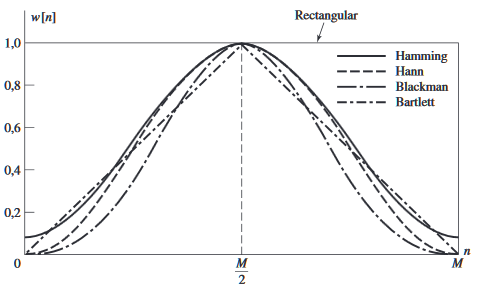
\includegraphics[width=10cm]{img/ventanas_grafica.png}
\caption{\label{fig:compven}Comparativa de las ventanas más utilizadas}
\end{center}
\end{figure}

Lógicamente, cuando aumentamos el factor de solapamiento más muestras procesamos y en consecuencia, menos eficiente es el algoritmo, puesto que se procesa información redundante. Este desperdicio de recursos en el procesado supone un compromiso doble con las prestaciones. Por un lado, cuanto más disminuya esta eficiencia, más aumentará la latencia, ya que habrá que esperar al cálculo de la siguiente trama para poder finalizar la construcción de la trama presente. Por otro lado, resulta mucho más complejo de cara a la implementación del flujo de datos resultante. 

Como conclusión, se debe elegir un factor de solapamiento $fs > 50$ para que resulte práctico, ya que si no el efecto es demasiado sutil como para que merezca la pena dedicar esfuerzo a su implementación en la arquitectura. Tras un modelado en Matlab, he implementado finalmente un valor de $fs = 75\%$ tal y como recomienda Ellis~\cite{Ellis} en su versión del vocoder de fase.

\begin{figure}[!b]
\begin{center}
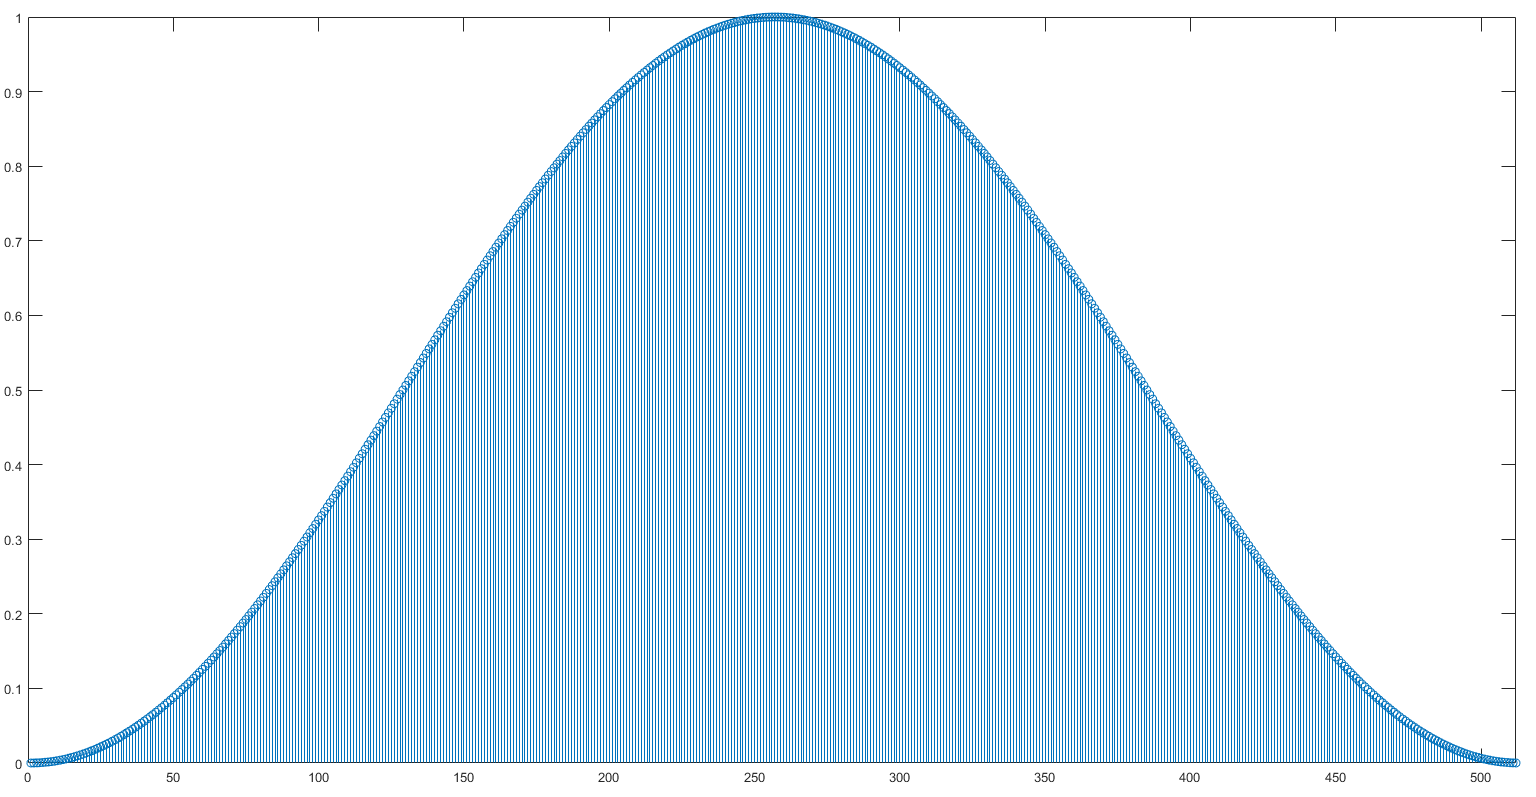
\includegraphics[width=14cm]{img/ventana_utilizada.png}
\caption{\label{fig:used_win}Ventana de Hann para $N = 512$ en Matlab}
\end{center}
\end{figure}

Como ya se ha visto antes, el solapamiento se utilizará junto con un enventanado de Hann cuya expresión se recoge en la ecuación~\ref{eq:Hann}. Esta ecuación resulta sencilla de implementar y su uso está muy extendido para aplicaciones de audio en tiempo real frente a algunas de sus alternativas mostradas en la figura~\ref{fig:compven}. El propio Ellis utiliza en su algoritmo~\cite{Ellis} una ventana de estas características.

\begin{equation}
\label{eq:Hann}
 H(n) = 0.5 * \left(1 - \cos\left(\frac{2\pi n}{N - 1}\right)\right)
 \end{equation} 
 
Estos mismos conceptos se utilizarán de forma completamente análoga en la etapa de la transformada inversa, tras introducir las muestras en el módulo iSTFT. La única excepción es que para mantener la amplitud de las muestras en la salida igual que las de la entrada, hay que aplicar un factor de escala de $2/3$. En la práctica, lo que se hará será aplicar este escalado a los propios coeficientes quedando una ventana de Hann reducida por el factor mencionado, permitiéndonos ahorrar una multiplicación y acelerar el flujo de datos a cambio de introducir otra memoria ROM.

\section{Operaciones sobre la fase}
A grandes rasgos este algoritmo opera dividiendo cada frecuencia entrante entre dos\footnote{El proceso recibe en \cite{Oppenheim} el nombre de \emph{diezmado}, en este caso por un valor 2.} y posteriormente modifica la fase para evitar el desplazamiento circular mencionado en \ref{nofourier}. El procesado se realiza por \emph{tramas consecutivas pares}: dos tramas se agrupan para formar una pareja de la que únicamente se va a poder calcular el valor de una sola trama de salida. De esta forma, la primera trama se agrupa con la segunda, la tercera con la cuarta y así sucesivamente.

\subsection{Cálculo del módulo}
El primer paso consiste en obtener el módulo de las muestras. Tras repasar el algoritmo, se puede ver que solo es necesario calcular este valor para una de cada dos muestras, ya que la otra es la que será diezmada y por tanto, no merece la pena malgastar recursos en esta operación. 

El cálculo del módulo a partir de la forma binomial es sencillo: $mod = \sqrt{re^{2}+im^{2}}$ donde $re$ es la parte real e $im$ la imaginaria. Sin embargo, la implementación en FPGA de una raíz cuadrada no resulta inmediata. Una opción es utilizar un módulo de cálculo como el CORDIC que procese los datos y devuelva la función raíz, mientras que otra es utilizar $lookup~tables$ para consultar el resultado de unas entradas previamente definidas. Este último método no es práctico ya que el tamaño de la memoria ROM que almacenaría esos datos sería demasiado grande, además Vivado proporciona los módulos IP que realizan estas operaciones matemáticas, entre otras, a cambio de unos pocos ciclos de procesado.

En esta ocasión, resulta más práctico realizar una aproximación que permita reducir el tamaño en área de la implementación así como la latencia de la misma, tal y como señala el doctor P.Chu en \cite{vhdlchu}. Si aproximamos por tanto según \ref{eq:mod_app}, donde $x~=~max\{|a|,|b|\}$ e $y~=~min\{|a|,|b|\}$, logramos simplificar en gran medida esta operación utilizando solo operaciones sencillas.

\begin{equation}
\label{eq:mod_app}
 \sqrt{a^{2}+b^{2}} \approx max\{((x - 0,125x) + 0,5y),x\}
\end{equation} 

\subsection{Recalculando la fase\label{calc_alg}}
Una vez obtenido el valor del módulo, se puede calcular la nueva fase de cada muestra teniendo en cuenta que se necesita la información de una trama $t$ y de la siguiente, $t+1$. El método para calcular la fase partiendo de la forma binomial es $\arctan(im/re)$ por lo que en este caso, si compensa utilizar un core IP de Vivado que realice esta operación para simplificar el diseño Además, otras operaciones trigonométricas serán necesarias más adelante.

Una vez calculada la fase de cada muestra entrante $n_{t}$, procedemos a obtener la fase de salida que se aplicará a cada muestra de salida $n_{t}'$. Para lo que calculamos una variable, $dp$, que se irá acumulando con $n$ según \ref{eq:phcalc}. 
\begin{equation}
\label{eq:phcalc}
dp = fase(n_{t+1}) - fase(n_{t}) - dphi
\end{equation} 
En esta fórmula se puede observar la existencia de una constante $dphi$ que habrá de valer $dphi~=~(\frac{n\pi}{2})$\footnote{Esta $n$ también se refiere al número de muestra dentro de una trama $t$. Hay que recordar que $0~\leq~n~\leq~puntos~de~la~transformada$, 511 en este caso} que se calcula aparte y se introduce en una ROM para utilizarla a lo largo del procesado (ver figura \ref{fig:esqalgoritmo}). Aunque pueda parecer que el valor resultante puede llegar a ser muy elevado debido al carácter de esta constante, el siguiente paso será reducirlo al intervalo $(-\pi,\pi)$, eliminando el problema.

Esta constante $dp$ va a servir para actualizar el valor de la fase \textbf{de la muestra siguiente $n+1$} operando según \ref{eq:phfin}, de forma que la fase de cada muestra depende de la anterior dentro de la misma trama. El valor calculado, se guardará en un registro destinado a tal fin.
\begin{equation}
\label{eq:phfin}
fase(n_{t}' + 1) = fase(n_{t}) + dp + dphi~~~~~~con~fase(n_{t}) = 0~~si~n=0
\end{equation} 

\begin{figure}[b]
\begin{center}
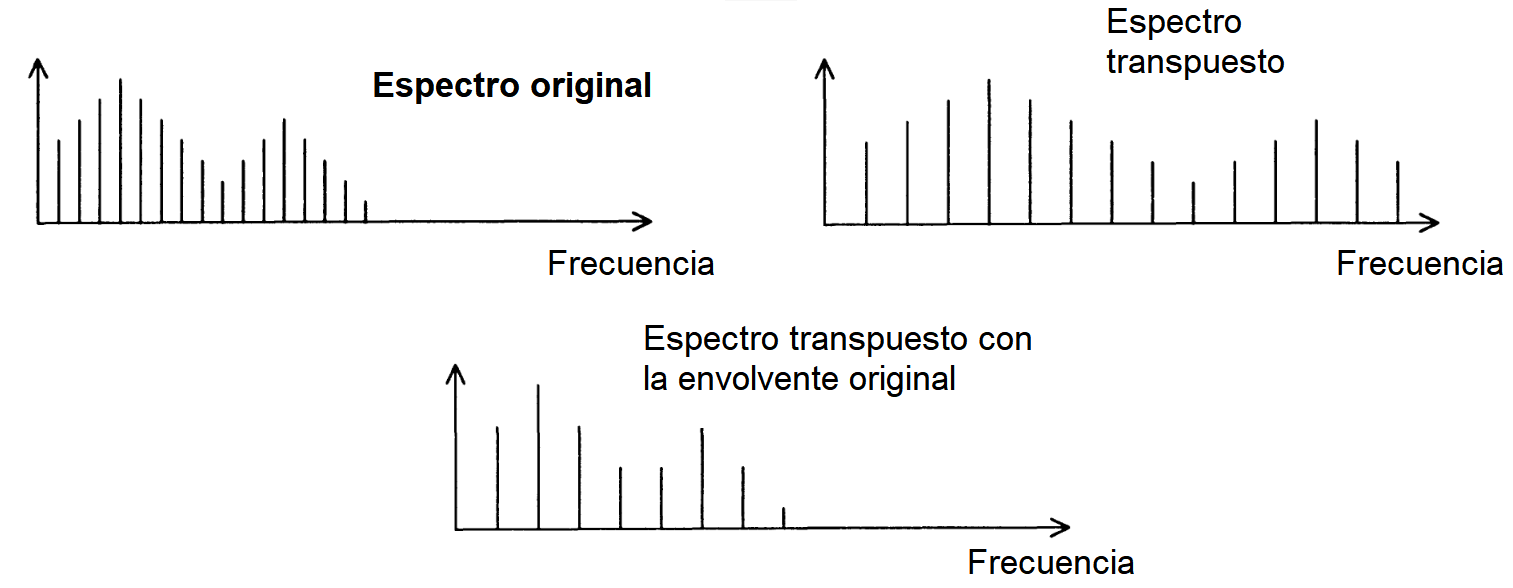
\includegraphics[width=14cm]{img/resample.png}
\caption{\label{fig:resample}Justificación de la necesidad de realizar el remuestreo}
\end{center}
\end{figure}

Tras este proceso, se prepara la muestra para iniciar la transformada inversa y posteriormente reenventanar la señal de salida cuando se procesen el resto de las muestras necesarias, como se ilustra en \ref{fig:esqalgoritmo}. Adicionalmente, es necesario remuestrear\footnote{Se ha utilizado esta palabra como traducción literal del término inglés \emph{resample}, que consiste en variar tasa de adquisión o lectura de muestras por factores enteros.} la señal resultante de la iFFT de forma que se irán insertando muestras nulas (ceros) en una de cada dos muestras procesadas, para conservar la duración del fragmento procesado en relación a la entrada. Al rellenar con ceros se introduce ruido un alta frecuencia, pero ni resulta audible para el oído humano, ni se va a llegar realmente a escribir en la salida, puesto que se realiza un filtrado paso bajo previamente. El proceso se muestra gráficamente en la figura \ref{fig:resample}. Esto no va a producir ningún efecto en la latencia puesto que la velocidad de procesado es mucho mayor que la frecuencia de muestreo.

\begin{figure}[!h]
\begin{center}
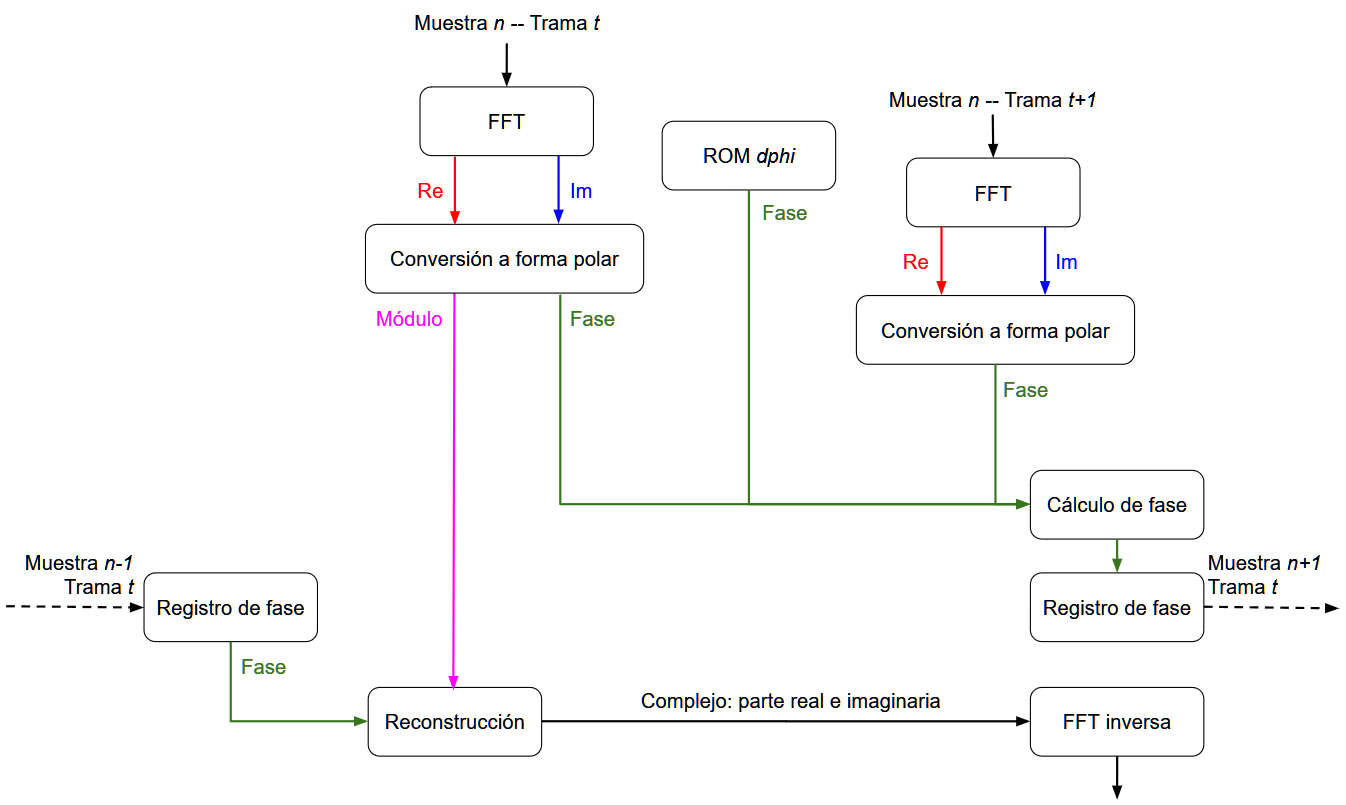
\includegraphics[width=15.5cm]{img/esq-alg.png}
\caption{\label{fig:esqalgoritmo}Diagrama de bloques del algortimo empleado}
\end{center}
\end{figure}

Para concluir, se puede afirmar que el algoritmo que se va a implementar es una adaptación del vocoder de fase propuesto por D.Ellis \cite{Ellis}, de forma que esté orientado directamente a la octavación y sea lo más adecuado posible para implementarlo sobre FPGA. A cambio de unos pocos ciclos más de latencia, consigue simplificar el diseño del flujo de datos que será implementado en la FPGA. Además, no hay que olvidar que se trata del algoritmo más usado en el mundo comercial precisamente por su sencillez.

